\section{Teorien: sju proposisjonar}
\label{sec:theory-nn}

Teorien er presentert som sju nummererte proposisjonar med underproposisjonar. Kvar underproposisjon er merka: \textit{d} (definisjon), \textit{a} (postulat), \textit{t} (teorem) eller \textit{o} (observasjon). Definisjonar er stipulative; postulat er antekne og falsifiserbare; teorem følgjer deduktivt frå tidlegare proposisjonar; observasjonar er empiriske påstandar testbare mot korpuset. Tabell~\ref{tab:propositions} oppsummerer dei sju hovudproposisjonane og det formelle apparatet kvar introduserer. Proposisjon 1--4 er operasjonaliserte og testa mot korpuset i seksjon~\ref{sec:empirical-nn}. Proposisjon 5--7 introduserer agenten, omsorgen og multiskala-dynamikken; dei er formaliserte her, illustrerte gjennom utarbeidde døme i seksjon~\ref{sec:examples-nn}, og genererer falsifiserbare forskingsprogram i seksjon~\ref{sec:agenda-nn}, men er ikkje direkte testa i den noverande studien.

\subsection{Proposisjon 1: Formverda er alt som er tilfelle}

Teorien byrjar med ontologi. Eit \textbf{objekt} er den enklaste bestanddelen i ei form; udeleleg innanfor det valde analysenivået. Ein \textbf{konfigurasjon} er ei samansetjing av objekt; forma er strukturen til konfigurasjonen. Desse to definisjonane fester det analytiske substratet: teorien opererer på strukturelle relasjonar mellom delar, ikkje på delane sjølve.

\textbf{Morforommet} til ein klasse er mengda av alle hennar moglege konfigurasjonar \parencite{Raup1966, Mitteroecker2009}. Kvart realisert objekt okkuperer eitt punkt i dette rommet. Det empiriske morforommet er alltid ein projeksjon; forma eksisterer uavhengig av målinga. Denne distinksjonen er viktig: ein kvar empirisk analyse fangar eit delrom, aldri det fulle morforommet.

Klassen er definert ikkje av ein einskild funksjon men av ein delt \textbf{affordansestruktur} \parencite{Gibson1979}. Objekta i klassen tilbyr same konstellasjon av operasjonar til same konstellasjon av agentar. Ein stol tilbyr sitting til ein menneskekropp, stabling til ein kelner, transport til eit fraktselskap, visuell karakter til eit sosialt rom.

Affordansestrukturen set \textit{naudsynte men ikkje tilstrekkelege} vilkår for klassetilhøyrsle. Ein trone og ein toalettstol deler affordansen sitting, men tilhøyrer ulike klassar; ein krakk og ein stol deler dei fleste affordansane, men grensa mellom dei er delvis kulturell, ikkje reint affordansestrukturell. Institusjonelle, lingvistiske og kulturelle faktorar medbestemmer klassegrensene. Affordansestrukturen set ramma; seleksjonstrykka (proposisjon 2) fordelar innhaldet innanfor ho.

Morforommet ber algebraisk struktur. Formene er lukka under union (kombinasjon), differanse (subtraksjon) og transformasjon (rotasjon, translasjon, skalering). Lat $S$ vere ei mengd av former i eit euklidsk rom $E^n$, utstyrt med transformasjonsgruppa $\mathrm{Trans}(E^n)$:

\begin{center}\small
\begin{tabular}{@{}l@{\hspace{4mm}}l@{}}
$s_1 + s_2$ & union \\
$s_1 - s_2$ & differanse \\
$s_1 \!\cdot\! s_2 := s_1 - (s_1 - s_2)$ & snitt (avleidd) \\
$\tau(a) \leq s,\;\tau \!\in\! \mathrm{Trans}(E^n)$ & innleiring \\
\end{tabular}
\end{center}

\noindent Ei \textbf{innleiring} av $a$ i $s$ er ein transformasjon som plasserer $a$ i $s$, eventuelt rotert, flytta eller skalert. Innleiringa er ein eigenskap ved den noverande forma, uavhengig av korleis ho vart konstruert \parencite{Stiny1972, Stiny2006}. Denne algebraen definerer dei syntaktiske operasjonane som er tilgjengelege i morforommet.

Morforommet deler seg i tre regionar: \textbf{busette} (det historiske arkivet av realiserte former), \textbf{opne} (det tilstøytande moglege; tilgjengelege men uaktualiserte) og \textbf{forbodne} (utelukka av materielle, strukturelle eller energetiske vilkår). Forbodet følgjer vilkåra, ikkje regionen; ein materialinnovasjon kan opne ein tidlegare forboden region.

Desse tre regionane svarar til ein epistemisk partisjon inspirert av C-K-teori \parencite{Hatchuel2003, Hatchuel2009}: det \textbf{kjende} ($K$), det \textbf{tenkelege} ($C \setminus K$) og det utenkjelege. $K$ inneheld alle former kjende å verke eller svikte. $C \setminus K$ inneheld alle former som er tenkelege men der statusen er uavgjort. Design er rørsla mellom dei, styrt av fire operatorar:

\begin{center}\small
\begin{tabular}{@{}l@{\;\;}l@{\;\;}l@{}}
\textbf{Op.} & \textbf{Retn.} & \textbf{Verknad} \\[2pt]
$C \!\to\! C$ & partisjon & konseptet vert spesifisert \\
$C \!\to\! K$ & realisering & konseptet vert avgjort \\
$K \!\to\! K$ & deduksjon & ny kunnskap \\
$K \!\to\! C$ & konjunksjon & opnar nye konsept \\
\end{tabular}
\end{center}

\subsection{Proposisjon 2: Ikkje alle posisjonar er like sannsynlege}

Eit \textbf{seleksjonstrykk} endrar sannsynsfordelinga i morforommet. Trykket er ein gradient, inga regel. Det avgrensar kvar posisjonen \textit{ikkje} kan vere. Forma er det som står att når trykka har utelukka alt anna \parencite{Michl1995}.

Tre postulat avgrensar trykksystemet. For det fyrste: eit trykk som inkje utelukkar er inkje trykk; eit trykk som utelukkar alt unnateke éin region er determinisme; alle observerte trykk ligg mellom desse ytterpunkta. For det andre: fleire seleksjonstrykk verkar samstundes; hadde berre eitt trykk eksistert, ville alle former innanfor klassen vore identiske. For det tredje: minst to trykk peikar i motstridande retningar; kvar realisert form er difor eit kompromiss. Omgrepet «suboptimal» føreset ein referanse; utan eit spesifisert trykksett er det ikkje falsifiserbart.

Affordansestrukturen definerer klassen (proposisjon 1), så han er konstant innanfor klassen og ber null informasjon om kvifor éi form oppstod framfor ei anna. All formvariasjon innanfor ein klasse er driven av dei resterande seleksjonstrykka. Dette er empirisk testbart: dersom stil (ein aggregert variabel som fangar det fulle trykksettet minus affordansen) predikerer meir formvariasjon enn materiale (eitt mekanisk trykk), kan ikkje bruk åleine vere den drivande krafta. Seksjon~\ref{sec:empirical-nn} stadfestar denne prediksjonen.

\textbf{Materialaffordansen} er operasjonane materialet tillèt og hindrar \parencite{Gibson1979}. Signaturen er latent: han bind sannsynsfordelinga utan å tvinge geometrien. Stål fanst i hundreår før røyrstolen fordi operasjonen (kaldbøying frå sykkelproduksjon) mangla. Formhistoria er systematisk langsamare enn materialhistoria.

\subsection{Proposisjon 3: Seleksjonstrykka produserer eit landskap}

\textbf{Tilpassingslandskapet} er vektorsummen av alle verksame seleksjonstrykk \parencite{Wright1932, Waddington1957}. Kvar posisjon i morforommet held ein verdi: graden av samtidig forløysing for alle trykk.

Landskapet kan berre loddast retrospektivt. Det yter lokal prediksjon, men inga einskildform er garantert. Fitnessfunksjonen har talrike lokale maksima; landskapet er eit taggete massiv, ikkje ein einaste topp. Éin universell topp er eit teoretisk unntak; empirien knuser postulatet om den eine perfekte forma \parencite{Kauffman1993}.

Stabiliteten til ein haug svarar til brattleiken på dalveggane. Dominante trykk produserer \textbf{kanalisering}: dei faldar morforommet til tronge korridorar der visse geometriske dimensjonar er stramt avgrensa medan andre er frie \parencite{Waddington1957}. Resultatet er eit \textit{avgrensningshierarki}: somme formeigenskapar varierer lite over klassen, medan andre fluktuerer fritt. Forholdet mellom den mest avgrensa og den minst avgrensa dimensjonen er eit direkte mål på landskapets selektivitet.

Ein \textbf{stilart} er forma si sverming kring eit felles tyngdepunkt \parencite{Kubler1962}. Stilarten er ein sverm, ikkje ein kategori; grensene er naudsynleg uskarpe. Stilperiodar er gradientar, ikkje øyar. Dette er direkte testbart: hadde stilar vore diskrete kategoriar, ville silhouette-analyse i morforommet gjeve positive skårar. Seksjon~\ref{sec:empirical-nn} viser at silhouette-skårane er gjennomgåande negative ($s = -0{,}338$), noko som stadfestar at stilar er overlappande gradientar.

\subsection{Proposisjon 4: Landskapet er dynamisk}

Seleksjonstrykka kviler aldri. Haugar stig, søkk, flyttar seg, deler seg, smeltar saman. Optimal tilpassing er lokal i tid. Ein ny teknologi flyttar grensa for det forbodne; ein ny marknad endrar kva landskapet belønnar; eit nytt materiale utvidar operasjonsrommet.

Endringa er diskontinuerleg. Lange periodar med stase brotnar i brå skifte: radiasjon inn i ein ny region, deretter konvergens. Diskontinuiteten er signaturen til dynamikken, ikkje eit brot med han \parencite{ElredgeGould1972}.

Landskapet har \textbf{minne} \parencite{Arthur1994}. Kvar realisert form endrar seleksjonstrykka for den neste. All design er redesign; agenten arvar alltid ein posisjon. Stiavhengigheit er eit fundamentalt trekk, ingen anomali.

Morforommet ekspanderer kumulativt. Det \textbf{tilstøytande moglege} er $C \setminus K$-grensa: mengda av former som er tenkelege men ikkje kjende som realiserbare \parencite{Kauffman1993}. Materialstraumar driv landskapsendringa. Når eitt trykk dominerer, kollapsar landskapet mot éin attraktor. Eit eineveldande trykk forklarer ikkje form; det er fråværet av forklaring. Diversitet speglar mangfald av aktive trykk.

Ei lære som reduserer alle seleksjonstrykk til eitt kollapsar den kognitive lyskjegla til éin dimensjon. Dette er ikkje rasjonalitet; det er redusert omsorg. Formene som oppstår under eit kollapsa landskap sviktar under dei reelle trykka læra var blind for. Skaden er i praksis irreversibel: dei fortrengde kompetansane; materialkulturane, handverkstradisjonane, dei lokale agentane; let seg ikkje gjenskape identisk frå læra som fortrengte dei.

\subsection{Proposisjon 5: Det finst agentar}

Kvar klasse har minst eitt system som navigerer landskapet via negativ tilbakekopling.

Ein \textbf{agent} er ein operator definert av trippelet: måltilstand, avstandsmåling, justeringsmekanisme \parencite{Rosenblueth1943, Wiener1948, Ashby1956}. Agens krev berre organisering; verken medvit, intensjon eller nervesystem. Informasjonsflyt skil agentar frå passiv materie. Definisjonen er substrat-uavhengig: eit kvart system som oppfyller vilkåra er ein agent.

Formelt. Ein agent $A := (g, d, \delta)$ tillet ein Lyapunov-funksjon $V$ slik at $V(g) = 0$, $V(x) > 0$ for $x \neq g$, og $V$ er ikkje-aukande langs trajektorien $x_{n+1} = \delta(x_n)$. Systemet nærmar seg målet. Agens er stratifisert: termostaten og arkitekten skil seg berre i navigasjonskompleksitet.

Den \textbf{kognitive lyskjegla} er delmengda av morforommet agenten kan representere og manipulere \parencite{Fields2022}. Alt utanfor lyskjegla manglar kausal eksistens for agenten. Lyskjegler spenner frå cellulær millisekundrespons til tiårslang konsensus.

Agenten manipulerer formgeometrien direkte. Konfigurasjonar lukka under union og differanse utgjer ein formalgebra; \textbf{formgrammatikken} \parencite{Stiny1972} utfører diskrete overgangar i denne geometrien. Ein formgrammatikk er eit trippel $SG = (S, R, \omega)$ der $R = \{r_i : (a_i, b_i)\}$:

\begin{center}\small
\begin{tabular}{@{}l@{\;\;}l@{}}
\textbf{Regel} & $s \!\to\! (s - \tau(a_i)) + \tau(b_i)$ \\[2pt]
\textbf{Språk} & $L(SG) = \{s \!\in\! S : \omega \!\to^*\! s\}$ \\[2pt]
\textbf{Fyring} & for kvar innleiring av $a_i$ i $s$ \\
\textbf{Premiss} & noverande geometri berre \\
\end{tabular}
\end{center}

\noindent Grammatikkoperasjonen er ein $C \to C$-partisjon: ho utvidar tanken. Realisering er ein $C \to K$-operasjon: ho avgjer han. Grammatikken definerer moglegheitsrommet; landskapet fastset trajektorien.

\textbf{Omsorg} er mengda av aksar i morforommet agenten aktivt representerer og justerer for \parencite{Doctor2024}. Ein agent med omsorg for tre dimensjonar oppdagar kompromiss ein agent med éin dimensjon ikkje veit finst. Den fyrste produserer former som toler fleire trykk samstundes. Den andre produserer former som sviktar langs dei aksane ho ikkje såg.

Omsorg er ikkje det same som \textit{kapasitet}. Kapasiteten til ein agent er bredda på lyskjegla; det er kor mange aksar agenten \textit{kan} representere. Omsorgen er kor mange han \textit{faktisk} representerer. Ein designar med brei kapasitet som likevel berre attenderer til éin akse; til dømes visuell nyheit åleine; viser trong omsorg trass i høg kapasitet. Distinksjonen er avgjerande for proposisjon 7: det er omsorgen, ikkje kapasiteten, som er leseleg i forma.

Ordet «omsorg» er valt medvite framfor «merksemd» eller «omfang». Merksemd er verdinøytralt; omsorg ber normativ vekt \parencite{Doctor2024}. Doctor, Wakefield, Pavlic og Levin avleier omgrepet frå buddhistisk medkjensletradisjon: omsorg inneber at agenten \textit{bør} representere fleire aksar, ikkje berre at han \textit{kan}. Denne normative dimensjonen er ikkje ei svakheit ved definisjonen; han er ein konsekvens av at designhandlinga har reelle konsekvensar langs dei aksane agenten vel å ikkje sjå.

Kompetansen til ein agent er evna til å navigere mot stabile posisjonar i landskapet. Kompetansen veks med omsorgen. Det me kallar intelligens, er nettopp denne kompetansen. Omsorg er intelligensen sitt innhald; intelligens er omsorgen si form \parencite{Doctor2024}.

\subsection{Proposisjon 6: Forma oppstår mellom agentane}

Fleire agentar responderer på ulike trykk samstundes. Kvar form er eit \textbf{poly-agentisk kompromiss}. Ingen einskild agent dikterer morfologien; ho trer fram i skjeringspunktet mellom dei.

Agens er \textbf{multiskalar} \parencite{Levin2022}. Kvar skala har sin eigen kompetanse og si eiga kognitive lyskjegle. Formproduksjon er distribuert $C \leftrightarrow K$-ekspansjon utført av grammatikkoperasjonar over kompetanseskalaer:

\begin{equation*}
\mathrm{Form} = SG\!\left(\nabla_{C(A)}\, L(c,\, t)\right)
\end{equation*}

\noindent der $SG$ er formgrammatikken, $L(c,t)$ er det skalare tilpassingslandskapet for klasse $c$ ved tid $t$, og $\nabla_{C(A)} L$ er gradienten av $L$ projisert ned på delrommet spent ut av agenten si kognitive lyskjegle $C(A)$. Formelt: dersom $\Pi_{C(A)}$ er den ortogonale projeksjonen på $C(A) \subseteq \mathbb{R}^n$, så er $\nabla_{C(A)} L = \Pi_{C(A)}\, \nabla L$. Agenten oppfattar berre dei komponentane av landskapsgradienten som fell innanfor hans representasjonskapasitet. Forma er grammatikken sin respons på denne oppfatta gradienten.

Ein presisjon er naudsynt. Likninga er eit \textit{strukturelt skjema}, ikkje ein prediksjonsmotor. Ho spesifiserer kva komponentar som er naudsynte og saman tilstrekkelege for å forklare form; grammatikk, landskap, og lyskjegle; men ho spesifiserer ikkje den funksjonelle forma til $L$, ikkje kva grammatikkreglar som fyrer, og ikkje dimensjonaliteten til $C(A)$ for ein gjeven agent. Analogien er $F = ma$ før kraftlova er kjend: Newton sin andre lov seier at kraft, masse og akselerasjon er dei rette komponentane, men predikerer ikkje bana til eit prosjektil utan at gravitasjonsfeltet er spesifisert. På same vis seier kjerne-likninga at form oppstår i skjeringspunktet mellom grammatikk, landskapsgradient og lyskjegle, men ein fullstendig prediktiv teori krev spesifikasjon av landskapsfunksjonen $L$ og lyskjegla $C(A)$. Den noverande studien legg det strukturelle grunnlaget; den parametriske spesifikasjonen er eit ope forskingsprogram (seksjon~\ref{sec:agenda-nn}).

Tabell~\ref{tab:ck-mapping} viser korleis C-K-operatorane kartlegg til landskapsnavigasjon og grammatikkoperasjonar. Dei to fyrste operatorane ($C \to C$ og $C \to K$) er direkte innlemma i kjerne-likninga. Dei to siste ($K \to K$ og $K \to C$) opererer på landskapet sjølv: deduksjon endrar agenten sin modell av landskapet utan å flytte posisjonen i morforommet, og konjunksjon opnar nye regionar av morforommet gjennom overraskande kunnskapssamanstillingar. Saman utgjer dei fire operatorane den epistemiske dynamikken som driv navigasjonen.

\begin{table}[!t]
\centering
\caption{Kartlegging av C-K-operatorar til landskapsnavigasjon.}
\label{tab:ck-mapping}
\small
\begin{tabularx}{\columnwidth}{@{}l l >{\raggedright\arraybackslash}X@{}}
\toprule
\textbf{Op.} & \textbf{C-K} & \textbf{Landskapstolking} \\
\midrule
$C \!\to\! C$ & partisjon & Grammatikkregel fyrer; ny posisjon i morforommet \\[2pt]
$C \!\to\! K$ & realisering & Prototypen vert bygd; konseptet får sannheitsverdi \\[2pt]
$K \!\to\! K$ & deduksjon & Landskapsmodellen vert oppdatert; gradienten vert klarare \\[2pt]
$K \!\to\! C$ & konjunksjon & Ny kunnskap opnar forbodne regionar; morforommet ekspanderer \\
\bottomrule
\end{tabularx}
\end{table}

Agenten vel; landskapet filtrerer. Kontrollen er alltid delt. Designaren er aldri åleine i landskapet. Ho navigerer i eit felt av konkurrerande agens frå mikrobielt vev til marknadskrefter \parencite{Levin2022}. Kompetansen hennar ligg i å koordinere uavhengige lyskjegler mot eit stabilt form-optimum.

Ein stilart manglar kausal kraft \parencite{Kubler1962, Michl1995}. Han er ikkje ei kraft men eit \textbf{mønsterminne}: ein makroskala-attraktor som kanar lyskjeglene til agentane som observerer han. Han forenklar navigasjon ved å tilby eit gjenkjenneleg tyngdepunkt; men å formgje «i ein stil» er ein kategorifeil; det er å imitere det statistiske utfallet av krefter ein ikkje har forstått.

Inga form er endeleg. Kvar balanse vert med tida suboptimal. Berre den generative strukturen varer: morforom, trykk, landskap, agentar. Formene er flyktige spor; grammatikken er stabil.

\subsection{Proposisjon 7: Forma viser kor langt omsorgen rakk}

Den avsluttande proposisjonen følgjer deduktivt frå proposisjon 5 og 6. Ho inneheld to påstandar som må skiljast.

\textbf{Den deskriptive påstanden} (teorem). Dersom omsorg er talet på aksar som er aktivt representerte (proposisjon 5), og dersom forma oppstår som eit poly-agentisk kompromiss over desse aksane (proposisjon 6), så er den realiserte forma eit leseleg arkiv over kompromisset sin dimensjonalitet. Forma er evidens. Gjeve ein realisert artefakt, predikerer teorien at sviktmønstra vil klyngje seg på aksar som var fråverande frå designaren si kognitive lyskjegle. Ei form designa under trong omsorg sviktar systematisk langs dei aksane som ikkje vart tekne vare på; svikten ber signaturen av blindskapen som produserte ho. Denne påstanden er falsifiserbar: dersom former designa under demonstrerbart trong omsorg ikkje presterer dårlegare langs urepresenterte aksar enn former designa under brei omsorg, er proposisjonen tilbakevist.

\textbf{Den normative påstanden} (etisk implikasjon). Dersom designaren kunne ha representert fleire aksar men valde å ikkje gjere det, er dei resulterande sviktane tilskrivbare det valet. Denne påstanden følgjer ikkje frå det formelle apparatet åleine; ho krev ein tilleggspremiss: at agentar bør representere så mange aksar som dei har kapasitet til. Premissen er ikkje deduserbar frå proposisjon 1--6, men han er heller ikkje vilkårleg; han følgjer av at designhandlinga har reelle konsekvensar for andre agentar som navigerer det same landskapet. Å snevra lyskjegla er å overlevere delar av formverda til krefter ingen representerer. Konsekvensane er borna av dei som lever med forma, ikkje av den som formgav ho.

Distinksjonen mellom desse to påstandane er viktig. Den deskriptive påstanden kan testast empirisk uavhengig av den normative. Den normative påstanden gjev den deskriptive retning og relevans, men står ikkje og fell med henne.

Figur~\ref{fig:levin-clc} illustrerer den kognitive lyskjegla slik Doctor et al. formaliserer ho: tre arketypar av omsorgskjegler med aukande dimensjonalitet. Figur~\ref{fig:synthesis} viser korleis syntese-likninga sameinar dei tre kjeldetradisjonane.

\begin{figure}[!t]
\centering
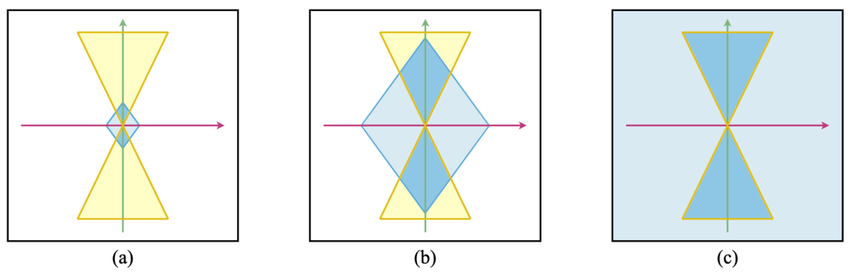
\includegraphics[width=\columnwidth]{figures/levin-clc-scales.png}
\caption{Tre arketypar av omsorgskjegler (CLC). \textbf{(a)}: Trong omsorg; agenten representerer få aksar. \textbf{(b)}: Moderat omsorg; agenten representerer fleire aksar enn den fysiske lyskjegla krev. \textbf{(c)}: Brei omsorg; agenten sin kognitive horisont overstig den fysiske rekkjevidda. Frå \textcite{Doctor2024}.}
\label{fig:levin-clc}
\end{figure}

\begin{figure}[!t]
\centering
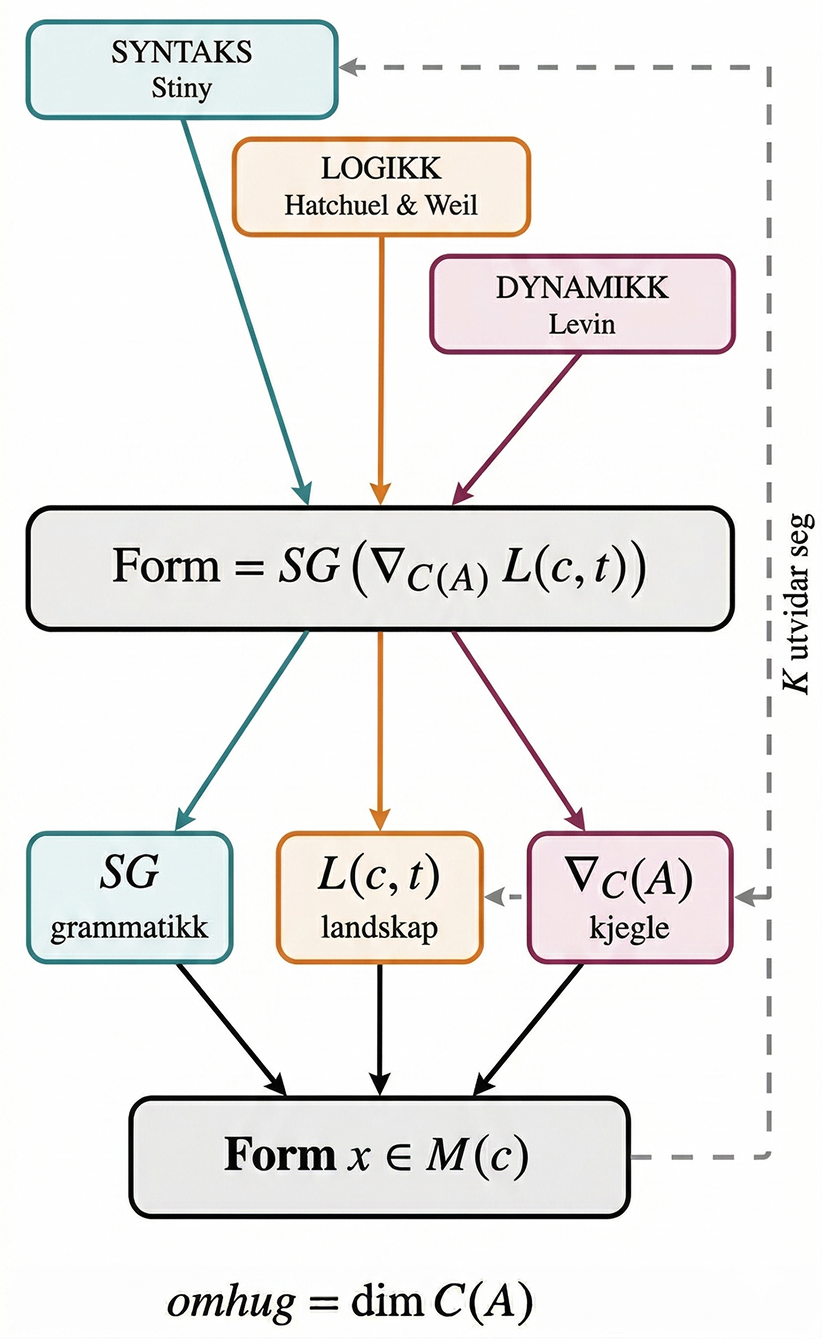
\includegraphics[width=0.70\columnwidth]{figures/syntese_diag_nn.png}
\caption{Syntese-likninga: tre kjeldetradisjonar (syntaks, logikk, dynamikk) konvergerer i kjerne-likninga $\mathrm{Form} = SG(\nabla_{C(A)} L(c,t))$. Stipla pil viser $K$-ekspansjonstilbakekopling.}
\label{fig:synthesis}
\end{figure}

\begin{table*}[!t]
\centering
\caption{Dei sju hovudproposisjonane i \formlaere{} med formelt apparat introdusert av kvar.}
\label{tab:propositions}
\small
\begin{tabularx}{\textwidth}{@{}c >{\raggedright}p{0.28\textwidth} >{\raggedright}p{0.32\textwidth} >{\raggedright\arraybackslash}p{0.22\textwidth}@{}}
\toprule
\textbf{Nr.} & \textbf{Proposisjon} & \textbf{Formelt apparat} & \textbf{Kjeldetradisjon} \\
\midrule
1 & Formverda er alt som er tilfelle & Morforom, algebra, $C$-$K$-partisjon & Stiny; Hatchuel \& Weil \\[3pt]
2 & Ikkje alle posisjonar er like sannsynlege & Seleksjonstrykk, affordanse & Gibson; Michl \\[3pt]
3 & Trykka produserer eit landskap & Tilpassingslandskap, kanalisering & Wright; Waddington \\[3pt]
4 & Landskapet er dynamisk & Stiavhengigheit, tilstøytande mogleg & Arthur; Kauffman \\[3pt]
5 & Det finst agentar & $A := (g,d,\delta)$;\; omsorg $= \dim C(A)$ & Levin; Doctor et al. \\[3pt]
6 & Forma oppstår mellom agentane & $\mathrm{Form} = SG(\nabla_{C(A)} L)$ & Syntese \\[3pt]
7 & Forma viser kor langt omsorgen rakk & Diagnostisk konklusjon & --- \\
\bottomrule
\end{tabularx}
\end{table*}

\begin{table}[!t]
\centering
\caption{Notasjonsoversikt.}
\label{tab:notation}
\small
\begin{tabularx}{\columnwidth}{@{}l >{\raggedright\arraybackslash}X@{}}
\toprule
\textbf{Symbol} & \textbf{Tyding} \\
\midrule
$M(c)$ & Morforommet til klasse $c$: mengda av alle moglege konfigurasjonar \\[2pt]
$S$ & Mengd av former i euklidsk rom $E^n$ \\[2pt]
$\mathrm{Trans}(E^n)$ & Transformasjonsgruppa (rotasjon, translasjon, skalering) \\[2pt]
$\tau(a) \leq s$ & Innleiring: $a$ kan finnast i $s$ under transformasjon $\tau$ \\[2pt]
$C$ & Tankerom: proposisjonar med uavgjort sannheitsverdi \\[2pt]
$K$ & Kunnskapsrom: proposisjonar med kjend sannheitsverdi \\[2pt]
$A := (g,d,\delta)$ & Agent: måltilstand, avstandsmål, justeringsmekanisme \\[2pt]
$C(A)$ & Kognitiv lyskjegle: delrommet agenten kan representere \\[2pt]
$\dim C(A)$ & Omsorg: talet på aksar agenten aktivt representerer \\[2pt]
$SG = (S,R,\omega)$ & Formgrammatikk: former, reglar, startsymbol \\[2pt]
$L(c,t)$ & Tilpassingslandskap for klasse $c$ ved tid $t$ \\[2pt]
$\nabla_{C(A)} L$ & Landskapsgradienten projisert på lyskjegla \\[2pt]
$\Pi_{C(A)}$ & Ortogonal projeksjon ned på $C(A)$ \\
\bottomrule
\end{tabularx}
\end{table}
